\documentclass[11pt,a4paper]{article}
\usepackage[utf8]{inputenc}
\usepackage[vietnamese]{babel}
\usepackage{amsmath,amssymb}
\usepackage[version=4]{mhchem}
\usepackage{geometry}
\geometry{top=1.1cm,bottom=1.0cm,left=1.4cm,right=1.4cm,headheight=24pt,headsep=7pt,footskip=13pt}
\usepackage{graphicx}
\usepackage{xcolor}
\usepackage{tabularx}
\usepackage{array}
\usepackage{tikz}
\usepackage{multicol}
\usepackage{fancyhdr}
\usepackage{enumitem}

\definecolor{hfRed}{HTML}{D32F2F}
\definecolor{hfGreen}{HTML}{8BC390}
\definecolor{mainGreen}{HTML}{2E7D32}

\usepackage{ex_test}

\pagestyle{fancy}
\fancyhf{}
\renewcommand{\headrulewidth}{0.75pt}
\renewcommand{\headrule}{\hbox to\headwidth{\color{hfGreen}\leaders\hrule height \headrulewidth\hfill}}
\renewcommand{\footrulewidth}{0.75pt}
\renewcommand{\footrule}{\hbox to\headwidth{\color{hfGreen}\leaders\hrule height \footrulewidth\hfill}}

\fancyhead[L]{\small\itshape\color{hfRed}Tài liệu lưu hành nội bộ}
\fancyhead[R]{\small\color{hfRed}Thầy \textbf{TRẦN VĂN THẠNH} - 0777.470.803}

\fancyfoot[L]{\footnotesize\itshape\color{hfRed}CS1: 6/15 Nguyễn Hoàng, P. Kim Long, TP Huế \quad|\quad CS2: 24 Đặng Thái Thân, TP Huế}
\fancyfoot[R]{\small\textbf{\color{hfRed}Trang \thepage}}

\setlength{\parindent}{0pt}
\setlength{\parskip}{1.2pt}

\def\loigiai#1{
\par\begingroup\color{blue!80!black}\small
\noindent\textbf{\textit{Lời giải chi tiết:}}\par
#1\par\endgroup}

\begin{document}

\Opensolutionfile{ans}[ans-de12-gv]

\noindent
\begin{minipage}[t]{0.48\textwidth}
	\textbf{SỞ GIÁO DỤC VÀ ĐÀO TẠO THỪA THIÊN HUẾ}\\
	\textbf{TRƯỜNG THPT HAI BÀ TRƯNG}\\
	\textbf{ĐỀ CHÍNH THỨC}\\
	\textit{(Đề thi có 04 trang)}
\end{minipage}\hfill
\begin{minipage}[t]{0.48\textwidth}
	\raggedleft
	\textbf{\color{mainGreen}ĐỀ KIỂM TRA ĐỊNH KỲ CHƯƠNG 4 (POLYMER)}\\
	\textbf{MÔN: HOÁ HỌC -- LỚP 12}\\
	\textit{Thời gian làm bài: 50 phút (không kể thời gian phát đề)}\\
	\textbf{Mã đề thi: 112}
\end{minipage}


\vspace{0.1cm}
\begin{center}
	\textbf{\color{hfRed}\Large (BẢN GIÁO VIÊN -- CÓ LỜI GIẢI CHI TIẾT)}
\end{center}

\vspace{0pt}
\noindent\textit{Họ, tên thí sinh: \dots\dots\dots\dots\dots\dots\dots\dots\dots\dots\dots\dots\dots\dots\dots\dots\dots\dots\dots\dots\dots\dots Lớp: \dots\dots\dots\dots SBD: \dots\dots\dots\dots}\\
\noindent\textit{(Cho biết nguyên tử khối: H = 1; C = 12; N = 14; O = 16; Na = 23; Al = 27; S = 32; Cl = 35,5; K = 39; Ca = 40; Fe = 56; Cu = 64; Zn = 65; Br = 80; Ag = 108; Ba = 137).}

\vspace{1pt}
\noindent
\textbf{PHẦN I (4,5 điểm -- 18 câu): Câu trắc nghiệm nhiều phương án lựa chọn.}\\
\textit{Thí sinh trả lời từ câu 1 đến câu 18. Mỗi câu hỏi thí sinh chỉ chọn một phương án.}

\setcounter{ex}{0}

\begin{ex}
Tên gọi của polymer có công thức cho dưới đây là
\par{\centering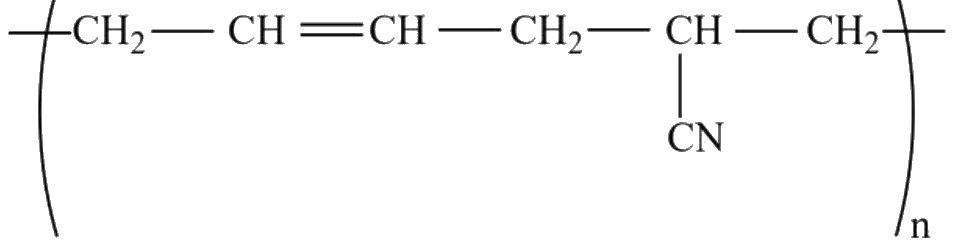
\includegraphics[height=0.8cm]{images_crop_de12/cau1_buna_n.png}\par}
\choice
{Cao su buna}
{Cao su buna-S}
{\True Cao su buna-N}
{Cao su isoprene}
\loigiai{
Phân tử polymer chứa mắt xích buta-1,3-diene (\ce{-CH2-CH=CH-CH2-}) kết hợp với mắt xích acrylonitrile (\ce{-CH(CN)-CH2-}), là sản phẩm đồng trùng hợp giữa buta-1,3-diene và acrylonitrile, có tên gọi là cao su buna-N (cao su nitrile, NBR).\\
\textbf{Chọn C.}}
\end{ex}

\begin{ex}
(SBT -- KNTT). Poly(vinyl chloride) (PVC) là một loại chất dẻo phổ biến, được sử dụng làm vỏ dây điện, ống dẫn nước thải, áo mưa, vải giả da,\dots{} PVC có công thức cấu tạo là
\choice
{$[-CH_2-CH_2-]_n$}
{$[-CH_2-CH(CH_3)-]_n$}
{$[-CH_2-CH(C_6H_5)-]_n$}
{\True $[-CH_2-CH(Cl)-]_n$}
\loigiai{
Poly(vinyl chloride) (PVC) được điều chế bằng phản ứng trùng hợp vinyl chloride (\ce{CH2=CHCl}), có công thức cấu tạo là \ce{[-CH2-CH(Cl)-]_n}.\\
\textbf{Chọn D.}}
\end{ex}

\begin{ex}
Polymer nào sau đây có thể cộng với hydrogen chloride?
\choice
{Polyacrylonitrile}
{Polyethylene}
{\True Polyisoprene}
{Tinh bột}
\loigiai{
Polyisoprene (\ce{[-CH2-C(CH3)=CH-CH2-]_n}) còn chứa liên kết đôi \ce{C=C} trong mỗi mắt xích nên có khả năng tham gia phản ứng cộng với hydrogen chloride (\ce{HCl}).\\
\textbf{Chọn C.}}
\end{ex}

\begin{ex}
Trong các phản ứng giữa các cặp chất dưới đây, phản ứng nào làm giảm mạch polymer?
\choice
{Poly(vinyl chloride) + \ce{Cl2}}
{Cao su thiên nhiên + \ce{HCl}}
{\True Tinh bột + \ce{H2O} ($t^\circ$, \ce{H+})}
{Poly(vinyl acetate) + \ce{NaOH}}
\loigiai{
Phản ứng thủy phân tinh bột trong môi trường acid có đun nóng (\ce{H2O}, \ce{H+}, $t^\circ$) làm đứt gãy các liên kết $\alpha$-glycosidic giữa các mắt xích glucose, phân cắt mạch polysaccharide dài thành dextrin, maltose và cuối cùng là glucose, do đó làm giảm mạch polymer.\\
\textbf{Chọn C.}}
\end{ex}

\begin{ex}
(SBT -- KNTT). Polymer nào sau đây \textbf{không} thuộc loại chất dẻo?
\choice
{Poly(methyl methacrylate)}
{Poly(vinyl chloride)}
{Polystyrene}
{\True Polybuta-1,3-diene}
\loigiai{
Polybuta-1,3-diene là polymer có tính đàn hồi cao, thuộc loại vật liệu cao su (cao su buna), không phải chất dẻo.\\
\textbf{Chọn D.}}
\end{ex}

\begin{ex}
(SBT -- KNTT). LDPE là một chất dẻo dễ tạo màng, có tính dai bền nên được sử dụng làm túi nylon, màng bọc, bao gói thực phẩm. Trên các bao bì làm từ LDPE thường được in kí hiệu như hình bên. LDPE được tổng hợp từ monomer nào sau đây?
\par{\centering
\includegraphics[height=0.85cm]{images_crop_de12/cau6_ldpe_symbol.png}\par}
\choice
{\True \ce{CH2=CH2}}
{\ce{CH2=CH-CH3}}
{\ce{CH2=CH-C6H5}}
{\ce{CH2=CHCl}}
\loigiai{
LDPE (Low-Density Polyethylene) là polyethylene có tỉ trọng thấp, được tổng hợp bằng phản ứng trùng hợp ethylene (\ce{CH2=CH2}) ở áp suất cao.\\
\textbf{Chọn A.}}
\end{ex}

\begin{ex}
(SBT -- CTST). Nylon-6,6 thuộc loại tơ nào sau đây?
\choice
{Tơ polyester}
{Tơ bán tổng hợp}
{Tơ thiên nhiên}
{\True Tơ tổng hợp}
\loigiai{
Nylon-6,6 được điều chế bằng phản ứng trùng ngưng giữa hexamethylenediamine và adipic acid, là các monomer được tổng hợp hoàn toàn từ công nghiệp hóa chất, do đó nylon-6,6 thuộc loại tơ tổng hợp (polyamide).\\
\textbf{Chọn D.}}
\end{ex}

\begin{ex}
(SBT -- CTST). Loại polymer thiên nhiên nào có thành phần chính là cellulose?
\choice
{\True Bông}
{Tơ tằm}
{Len}
{Cao su thiên nhiên}
\loigiai{
Sợi bông (bông nõn) có thành phần chính là cellulose, chiếm khoảng 95\% - 98\% khối lượng. Tơ tằm và len cấu tạo từ protein; cao su thiên nhiên là polyisoprene.\\
\textbf{Chọn A.}}
\end{ex}

\begin{ex}
(SBT -- KNTT). Cao su buna-N (hay còn gọi là cao su nitrile, có kí hiệu là NBR) là loại cao su tổng hợp có khả năng chịu dầu mỡ tốt nên được dùng làm ống dẫn nhiên liệu, gioăng phớt làm kín trong các máy móc. Thực hiện phản ứng trùng hợp các chất nào dưới đây thu được sản phẩm là cao su buna-N?
\choice
{\ce{CH2=CH-CH=CH2} và \ce{C6H5CH=CH2}}
{\ce{CH2=C(CH3)-CH=CH2} và \ce{CH2=CHCN}}
{\ce{CH2=CH-CH=CH2} và \ce{N2}}
{\True \ce{CH2=CH-CH=CH2} và \ce{CH2=CHCN}}
\loigiai{
Cao su buna-N được điều chế bằng phản ứng đồng trùng hợp buta-1,3-diene (\ce{CH2=CH-CH=CH2}) và vinyl cyanide (acrylonitrile, \ce{CH2=CH-CN}) có xúc tác thích hợp.\\
\textbf{Chọn D.}}
\end{ex}

\begin{ex}
Nhận xét về tính chất vật lí chung của polymer nào dưới đây \textbf{không} đúng?
\choice
{Hầu hết là những chất rắn, không bay hơi}
{Đa số nóng chảy ở một khoảng nhiệt độ rộng, hoặc không nóng chảy mà bị phân hủy khi đun nóng}
{Đa số không tan trong các dung môi thông thường, một số tan trong dung môi thích hợp tạo dung dịch nhớt}
{\True Hầu hết polymer đều đồng thời có tính dẻo, tính đàn hồi và có thể kéo thành sợi dai, bền}
\loigiai{
Mỗi loại polymer có những đặc tính cơ học riêng biệt: chất dẻo có tính dẻo, cao su có tính đàn hồi, tơ sợi có thể kéo sợi dai bền. Hầu hết các polymer không đồng thời có cả 3 đặc tính cơ học trên. Do đó nhận xét D là không đúng.\\
\textbf{Chọn D.}}
\end{ex}



\begin{ex}
Dãy nào sau đây chỉ chứa các polymer thiên nhiên?
\choice
{Poly(vinyl chloride), tinh bột, cellulose}
{Protein, tinh bột, polyethylene}
{Protein, cellulose}
{\True Protein, tinh bột, cellulose}
\loigiai{
Protein, tinh bột và cellulose là các polymer có sẵn trong cơ thể sinh vật và thực vật tự nhiên nên đều thuộc loại polymer thiên nhiên. Các chất PVC và polyethylene là polymer tổng hợp.\\
\textbf{Chọn D.}}
\end{ex}

\begin{ex}
Cho dãy gồm các polymer: (1) polybuta-1,3-diene, (2) polyacrylonitrile, (3) poly(vinyl chloride), (4) poly(hexamethylene adipamide). Polymer bị thuỷ phân trong môi trường acid là
\choice
{(1)}
{(3)}
{\True (4)}
{(2)}
\loigiai{
(4) Poly(hexamethylene adipamide) (nylon-6,6) chứa các liên kết amide \ce{-CO-NH-} trong mạch phân tử, dễ bị thủy phân trong cả môi trường acid và kiềm. Các polymer còn lại chỉ có liên kết carbon--carbon bền vững ở mạch chính nên không bị thủy phân.\\
\textbf{Chọn C.}}
\end{ex}

\begin{ex}
Nhận xét nào sau đây đúng?
\choice
{Đa số các polymer dễ hòa tan trong các dung môi thông thường}
{\True Đa số các polymer không có nhiệt độ nóng chảy xác định}
{Các polymer đều bền vững dưới tác động của acid, base}
{Các polymer dễ bay hơi}
\loigiai{
Đa số các polymer là hỗn hợp của các phân tử có khối lượng và độ dài mạch khác nhau nên không có nhiệt độ nóng chảy xác định mà nóng chảy trong một khoảng nhiệt độ khá rộng.\\
\textbf{Chọn B.}}
\end{ex}

\begin{ex}
Cho các polymer sau: polyethylene, poly(methyl methacrylate), poly(vinyl chloride), polyacrylonitrile. Số polymer điều chế được bằng phản ứng trùng hợp là
\choice
{3}
{\True 4}
{1}
{2}
\loigiai{
Cả 4 polymer trên đều được điều chế bằng phản ứng trùng hợp monomer chứa liên kết đôi \ce{C=C}:\\
- Polyethylene từ \ce{CH2=CH2}.\\
- Poly(methyl methacrylate) từ \ce{CH2=C(CH3)-COOCH3}.\\
- Poly(vinyl chloride) từ \ce{CH2=CHCl}.\\
- Polyacrylonitrile từ \ce{CH2=CH-CN}.\\
\textbf{Chọn B.}}
\end{ex}

\begin{ex}
Phát biểu nào sau đây sai?
\choice
{Tơ nitron thuộc loại tơ tổng hợp}
{Tơ nylon-6,6 thuộc loại tơ tổng hợp}
{\True Tơ visco thuộc loại tơ thiên nhiên}
{Tơ acetate thuộc loại tơ bán tổng hợp}
\loigiai{
Tơ visco là tơ bán tổng hợp (tơ nhân tạo) được điều chế bằng con đường hóa học từ nguyên liệu thiên nhiên là cellulose, không phải là tơ thiên nhiên.\\
\textbf{Chọn C.}}
\end{ex}

\begin{ex}
Phát biểu sai là
\choice
{Bản chất cấu tạo hoá học của tơ tằm và len là protein; của sợi bông là cellulose}
{Bản chất cấu tạo hoá học của tơ nylon là polyamide}
{Quần áo nylon, len, tơ tằm không nên giặt với xà phòng có độ kiềm cao}
{\True Tơ nylon, tơ tằm, len rất bền vững với nhiệt}
\loigiai{
Tơ nylon, tơ tằm, len đều kém bền với nhiệt do chứa các liên kết amide/peptide dễ bị đứt gãy hoặc biến tính ở nhiệt độ cao, nếu là (ủi) quá nóng sẽ làm co rúm và hỏng sợi vải.\\
\textbf{Chọn D.}}
\end{ex}

\begin{ex}
(SBT -- CTST). Trùng ngưng $\varepsilon$-aminocaproic acid thu được $m\text{ kg}$ capron và $12{,}6\text{ kg } \ce{H2O}$ với hiệu suất phản ứng 90\%. Giá trị của $m$ là
\choice
{71,19}
{\True 79,10}
{91,70}
{90,40}
\loigiai{
Phương trình phản ứng trùng ngưng:
$$n\,\ce{H2N-(CH2)5-COOH} \xrightarrow{t^\circ} \ce{[-NH-(CH2)5-CO-]_n} + n\,\ce{H2O}$$
Theo phương trình: Cứ $n\text{ mol } \ce{H2O}$ sinh ra đồng thời với $1\text{ mol}$ mắt xích capron ($113n\text{ g}$).\\
Số mol \ce{H2O} thực tế thu được:
$$n_{\ce{H2O}} = \frac{12{,}6}{18} = 0{,}7\text{ kmol.}$$
Khối lượng capron thực tế thu được tương ứng là:
$$m = 0{,}7 \times 113 = 79{,}10\text{ kg.}$$
(Vì lượng \ce{H2O} cho trong đề là lượng thực tế sinh ra, nên lượng polymer thực tế tạo thành tỉ lệ trực tiếp theo stoichiometry là $79{,}10\text{ kg}$).\\
\textbf{Chọn B.}}
\end{ex}

\begin{ex}
Keo dán là vật liệu được sử dụng rộng rãi trong đời sống. Cho các phát biểu sau về keo dán:\\
(a) Keo dán là vật liệu có khả năng kết dính bề mặt của hai vật liệu rắn với nhau mà không làm biến đổi bản chất các vật liệu được kết dính.\\
(b) Nhựa vá săm là dung dịch dạng keo của chất dẻo trong dung môi hữu cơ như toluene, xylene, thường được dùng để vá chỗ thủng của săm xe.\\
(c) Keo dán epoxy còn gọi là keo dán một thành phần.\\
(d) Thành phần chính của keo epoxy là hợp chất chứa hai nhóm epoxy ở hai đầu. Thành phần thứ hai là chất đóng rắn, thường là các polyamine.\\
(e) Ưu điểm của keo epoxy là độ kết dính rất cao, chịu nhiệt, chịu nước, chịu dung môi, chịu lực tốt, rất dễ sử dụng. Keo epoxy thường được dùng để dán các kim loại, nhựa, bê tông, các vật bằng kính, sứ, gỗ, đồ gốm.\\
Số phát biểu đúng là
\choice
{2}
{\True 3}
{5}
{4}
\loigiai{
Các phát biểu đúng gồm 3 phát biểu: (a), (d), (e).\\
- (a) \textbf{Đúng}: Theo định nghĩa vật liệu keo dán.\\
- (b) \textbf{Sai}: Nhựa vá săm là dung dịch dạng keo của \textbf{cao su} trong dung môi hữu cơ, không phải chất dẻo.\\
- (c) \textbf{Sai}: Keo dán epoxy là loại keo dán \textbf{hai thành phần} (keo A và B).\\
- (d) \textbf{Đúng}: Gồm hợp chất chứa 2 nhóm epoxy và chất đóng rắn polyamine.\\
- (e) \textbf{Đúng}: Đây là các tính chất cơ lí ưu việt và phạm vi ứng dụng rộng rãi của keo epoxy.\\
\textbf{Chọn B.}}
\end{ex}



\noindent
\textbf{PHẦN II (4,0 điểm -- 4 câu): Câu trắc nghiệm đúng sai.}\\
\textit{Thí sinh trả lời từ câu 1 đến câu 4. Trong mỗi ý a), b), c), d) ở mỗi câu, thí sinh chọn đúng hoặc sai.}

\setcounter{ex}{0}

\begin{ex}
(SBT -- CTST). Tơ capron và polyacrylonitrile có công thức cấu tạo như hình dưới:
\par\vspace{1pt}{\centering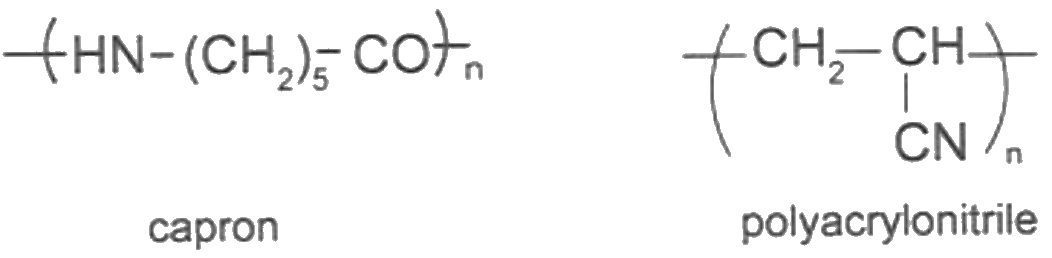
\includegraphics[height=1.0cm]{images_crop_de12/p2_cau1_polymers.png}\par}\vspace{1pt}
\choiceTF
{\True Cả hai loại đều dùng để chế tạo tơ}
{Polyacrylonitrile được điều chế bằng phản ứng trùng ngưng}
{Capron thuộc loại polypeptide}
{Hai polymer đều có phản ứng phân huỷ mạch trong môi trường kiềm}
\loigiai{
a) \textbf{Đúng}. Capron dùng làm tơ capron (nylon-6), polyacrylonitrile dùng làm tơ nitron (olon).\\
b) \textbf{Sai}. Polyacrylonitrile được điều chế bằng phản ứng trùng hợp monomer acrylonitrile (vinyl cyanide, \ce{CH2=CH-CN}).\\
c) \textbf{Sai}. Capron thuộc loại polyamide (polycaproamide), mắt xích tạo từ amino acid riêng biệt $\varepsilon$-aminocaproic acid, không phải là polypeptide (polypeptide gồm chuỗi nối từ các $\alpha$-amino acid).\\
d) \textbf{Sai}. Capron có liên kết amide \ce{-CO-NH-} bị thủy phân phân hủy mạch trong kiềm, nhưng polyacrylonitrile có mạch chính carbon--carbon bền vững nên không bị phân hủy mạch trong kiềm.}
\end{ex}

\begin{ex}
(SBT -- CĐ). Năm 1839, Charles Goodyear đã được cấp bằng sáng chế cho phát minh về quy trình hoá học để chế tạo ra cao su lưu hoá -- một loại cao su có cấu trúc đặc biệt, bền cơ học, chịu được sự ma sát, va chạm, đàn hồi tốt và có thể đúc được. Những phát biểu nào sau đây là đúng?
\choiceTF
{Cao su lưu hoá còn có tên gọi là cao su buna-S}
{\True Bản chất của việc lưu hoá cao su là tạo ra cầu nối disulfide \ce{-S-S-} giữa các mạch cao su nên cao su lưu hoá có tính chất cơ lí nổi trội hơn}
{\True Trong mủ cao su thiên nhiên, polymer có tính đàn hồi là polyisoprene}
{\True Cao su lưu hoá có cấu trúc mạng không gian nên bền hơn cao su chưa lưu hoá}
\loigiai{
a) \textbf{Sai}. Cao su buna-S là sản phẩm đồng trùng hợp buta-1,3-diene với styrene, khác với cao su lưu hóa (được chế tạo bằng phản ứng giữa cao su với lưu huỳnh).\\
b) \textbf{Đúng}. Cầu nối disulfide \ce{-S-S-} liên kết các mạch phân tử cao su tạo thành mạng không gian 3 chiều bền vững.\\
c) \textbf{Đúng}. Thành phần chính tạo nên tính đàn hồi của mủ cao su thiên nhiên là cis-polyisoprene.\\
d) \textbf{Đúng}. Cấu trúc mạng không gian giúp cao su lưu hóa có độ bền cơ học cao hơn, đàn hồi tốt hơn, chịu nhiệt và chống mài mòn vượt trội.}
\end{ex}

\begin{ex}
Cây cao su là loại cây công nghiệp có giá trị kinh tế lớn, được đưa vào trồng ở nước ta từ cuối thế kỉ 19. Chất lỏng thu được từ cây cao su giống như nhựa cây (gọi là mủ cao su) là nguyên liệu để sản xuất cao su tự nhiên.
\choiceTF
{\True Thành phần chính của cao su thiên nhiên là polyisoprene có cấu hình dạng cis}
{\True Cao su thiên nhiên có tính đàn hồi, không có tính dẫn điện, không thấm khí và nước, không tan trong nước, nhưng tan nhiều trong xăng, benzene\dots}
{Cao su thiên nhiên có tính đàn hồi chỉ tồn tại trong khoảng nhiệt độ hẹp. Để cải thiện tính chất này người ta xử lý bằng cách trộn cao su thiên nhiên với styrene gọi là quá trình lưu hóa cao su}
{\True Mắt xích của cao su thiên nhiên được viết thu gọn là \ce{C5H8}}
\loigiai{
a) \textbf{Đúng}. Cao su thiên nhiên là cis-1,4-polyisoprene.\\
b) \textbf{Đúng}. Đây là các tính chất vật lí đặc trưng của cao su thiên nhiên.\\
c) \textbf{Sai}. Quá trình lưu hóa cao su là đun nóng cao su thiên nhiên với lưu huỳnh (S), không phải styrene.\\
d) \textbf{Đúng}. Mắt xích polyisoprene có dạng \ce{[-CH2-C(CH3)=CH-CH2-]}, công thức thực nghiệm thu gọn là \ce{C5H8}.}
\end{ex}

\begin{ex}
Bản chất kết dính của keo dán là tạo ra lớp màng mỏng bám chắc vào hai mảnh vật liệu để giúp chúng kết dính lại với nhau.
\choiceTF
{\True Keo dán poly(urea -- formaldehyde) được điều chế từ phản ứng trùng ngưng}
{Keo dán poly(urea -- formaldehyde) gồm phần chính là poly(urea -- formaldehyde) và thêm phần đóng rắn như oxalic acid, ammonium chloride\dots{} để tạo polymer có cấu trúc mạch phân nhánh}
{\True Keo dán epoxy có polymer mạng không gian với độ kết dính cao dùng để gắn kết hai bề mặt vật cần dán lại như kim loại, thủy tinh, gỗ\dots}
{\True Keo dán tổng hợp thông dụng thường gặp gồm keo dán urea -- formaldehyde, keo dán epoxy và nhựa vá săm}
\loigiai{
a) \textbf{Đúng}. Keo poly(urea -- formaldehyde) được điều chế bằng phản ứng trùng ngưng giữa urea (\ce{NH2-CO-NH2}) và formaldehyde (\ce{HCHO}).\\
b) \textbf{Sai}. Chất đóng rắn xúc tác tạo mạng lưới polymer \textbf{mạng không gian}, không phải mạch phân nhánh.\\
c) \textbf{Đúng}. Keo epoxy tạo polymer cấu trúc mạng không gian bền chắc, có độ kết dính cao.\\
d) \textbf{Đúng}. Đây là ba loại keo dán tổng hợp phổ biến thường gặp trong đời sống và kĩ thuật.}
\end{ex}



\noindent
\textbf{PHẦN III (1,5 điểm -- 6 câu): Câu trắc nghiệm yêu cầu trả lời ngắn.}\\
\textit{Thí sinh trả lời từ câu 1 đến câu 6.}

\setcounter{ex}{0}

\begin{ex}
Cho dãy gồm các nguyên liệu: (1) $\varepsilon$-aminocaproic acid, (2) acrylonitrile, (3) $\omega$-aminoenanthic acid, (4) ethylene glycol và terephthalic acid, (5) hexamethylenediamine và adipic acid. Số nguyên liệu (hoặc cặp nguyên liệu) được dùng để tiến hành phản ứng trùng ngưng tạo thành tơ là
\par\noindent\textbf{Đáp số:} \textbf{\color{red}4}
\loigiai{
Có 4 nguyên liệu/cặp nguyên liệu dùng để trùng ngưng tạo tơ:\\
- (1) $\varepsilon$-aminocaproic acid $\rightarrow$ tơ capron (nylon-6).\\
- (3) $\omega$-aminoenanthic acid $\rightarrow$ tơ enang (nylon-7).\\
- (4) ethylene glycol và terephthalic acid $\rightarrow$ tơ lapsan (PET).\\
- (5) hexamethylenediamine và adipic acid $\rightarrow$ tơ nylon-6,6.\\
(Nguyên liệu (2) acrylonitrile dùng điều chế tơ nitron bằng phản ứng trùng hợp).\\
\textbf{Đáp số: 4.}}
\end{ex}

\begin{ex}
Cho các polymer: amylose (1); cao su isoprene (2); cellulose acetate (3); thủy tinh hữu cơ (4); tơ tằm (5). Số lượng polymer thiên nhiên là
\par\noindent\textbf{Đáp số:} \textbf{\color{red}2}
\loigiai{
Có 2 polymer thiên nhiên là: amylose (1) và tơ tằm (5).\\
(Cao su isoprene trong đề là cao su tổng hợp polyisoprene; cellulose acetate là polymer bán tổng hợp; thủy tinh hữu cơ là polymer tổng hợp).\\
\textbf{Đáp số: 2.}}
\end{ex}

\begin{ex}
Phân tử khối của một đoạn mạch tơ nylon-6,6 là 56 500 amu. Số lượng mắt xích trong đoạn mạch nylon-6,6 nêu trên là
\par\noindent\textbf{Đáp số:} \textbf{\color{red}250}
\loigiai{
Mắt xích tơ nylon-6,6 có công thức \ce{[-NH-(CH2)6-NH-CO-(CH2)4-CO-]} với phân tử khối:
$$M_{\text{mắt xích}} = 116 + 146 - 2 \times 18 = 226\text{ amu.}$$
Số lượng mắt xích trong đoạn mạch:
$$n = \frac{56500}{226} = 250.$$
\textbf{Đáp số: 250.}}
\end{ex}

\begin{ex}
Polystyrene (PS) là loại nhựa dùng chế tạo hộp xốp đựng thức ăn. Hãy tính hệ số polymer hóa của loại nhựa này khi biết phân tử khối của nó bằng 104 000 amu.
\par\noindent\textbf{Đáp số:} \textbf{\color{red}1000}
\loigiai{
Polystyrene có công thức \ce{[-CH2-CH(C6H5)-]_n} với phân tử khối của một mắt xích là $M = 104\text{ amu}$.\\
Hệ số polymer hóa là:
$$n = \frac{104000}{104} = 1000.$$
\textbf{Đáp số: 1000.}}
\end{ex}

\begin{ex}
Trong công nghiệp, để điều chế cao su buna người ta có thể đi từ nguyên liệu khí ethylene thu được từ dầu mỏ theo sơ đồ:
$$2\,\ce{C2H4} \xrightarrow{(1)} 2\,\ce{C2H5OH} \xrightarrow{(2)} \ce{C4H6} \xrightarrow{(3)} \ce{[-CH2-CH=CH-CH2-]_n}\text{ (cao su buna)}$$
Tính thể tích khí ethylene (đo ở 25 $^\circ\text{C}$ và 1 bar) cần lấy để điều chế được 1 tấn cao su buna theo sơ đồ trên. Giả sử hiệu suất phản ứng của mỗi quá trình (1), (2) và (3) lần lượt là 65\%, 50\% và 70\% (kết quả làm tròn đến hàng đơn vị theo đơn vị $\text{m}^3$).
\par\noindent\textbf{Đáp số:} \textbf{\color{red}4036}
\loigiai{
Khối lượng cao su buna: $m = 1\text{ tấn} = 1000\text{ kg}$.\\
Số mol mắt xích cao su buna:
$$n_{\text{cao su}} = \frac{1000}{54}\text{ kmol.}$$
Theo sơ đồ bảo toàn nguyên tố C, 1 mắt xích \ce{C4H6} cần 2 phân tử \ce{C2H4}:
$$n_{\ce{C2H4}\text{ (lý thuyết)}} = 2 \times \frac{1000}{54} = \frac{2000}{54}\text{ kmol.}$$
Hiệu suất tổng của quá trình:
$$H_{\text{tổng}} = 65\% \times 50\% \times 70\% = 0{,}65 \times 0{,}50 \times 0{,}70 = 0{,}2275 = 22{,}75\%.$$
Ở 25 $^\circ\text{C}$, 1 bar ($V_m = 24{,}79\text{ m}^3/\text{kmol}$), thể tích ethylene thực tế cần dùng là:
$$V_{\ce{C2H4}} = \frac{2000}{54 \times 0{,}2275} \times 24{,}79 \approx 4035{,}82 \approx 4036\text{ m}^3.$$
\textbf{Đáp số: 4036.}}
\end{ex}

\begin{ex}
(SBT -- CĐ). Caprolactam được tổng hợp từ cuối thế kỉ XIX. Hiện nay, nhu cầu sản xuất caprolactam trên thế giới khoảng 10 triệu tấn/năm; 90\% trong đó dùng để tổng hợp tơ capron. Trong công nghiệp, caprolactam được điều chế theo sơ đồ sau:
\par\vspace{2pt}{\centering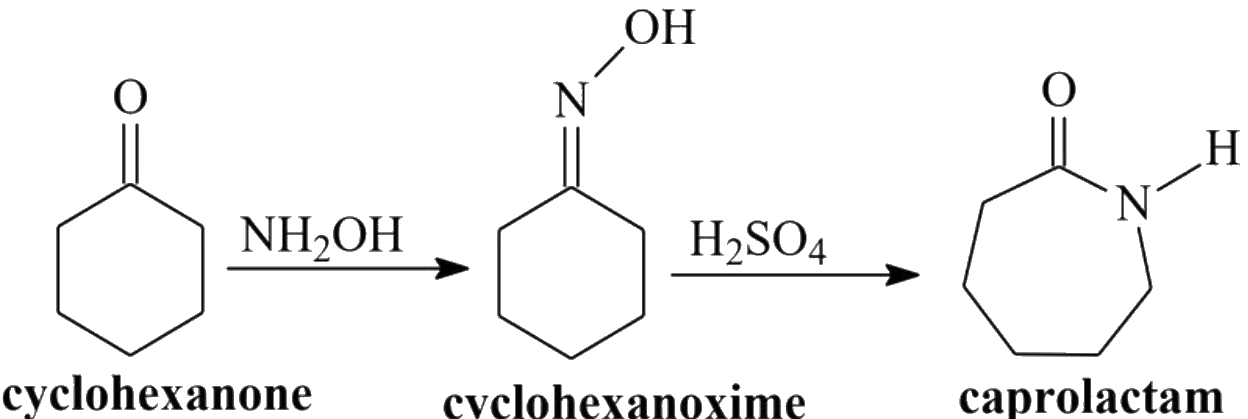
\includegraphics[height=1.8cm]{images_crop_de12/p3_cau6_caprolactam_scheme.png}\par}\vspace{2pt}
Để sản xuất 10 triệu tấn caprolactam, cần sử dụng bao nhiêu triệu tấn cyclohexanone (giả sử hiệu suất trung bình của cả quá trình trên là 60\%)? (Kết quả làm tròn đến chữ số hàng phần mười).
\par\noindent\textbf{Đáp số:} \textbf{\color{red}14,5}
\loigiai{
Sơ đồ chuyển hóa tổng quát:
$$\text{Cyclohexanone } (\ce{C6H10O},\ M = 98) \xrightarrow{H = 60\%} \text{Caprolactam } (\ce{C6H11NO},\ M = 113)$$
Số mol caprolactam cần sản xuất:
$$n = \frac{10}{113}\text{ triệu kmol.}$$
Khối lượng cyclohexanone cần dùng với hiệu suất 60\%:
$$m = \frac{10}{113} \times 98 \times \frac{100}{60} \approx 14{,}454 \approx 14{,}5\text{ triệu tấn.}$$
\textbf{Đáp số: 14,5.}}
\end{ex}


\Closesolutionfile{ans}

\vspace{0.5cm}
\begin{center}
	\textbf{\Large\color{mainGreen}BẢNG TỔNG HỢP ĐÁP ÁN ĐỀ SỐ 12}
\end{center}

\vspace{0.2cm}
\noindent\textbf{\color{mainGreen}PHẦN I: TRẮC NGHIỆM NHIỀU PHƯƠNG ÁN LỰA CHỌN}
\begin{center}
\renewcommand{\arraystretch}{1.2}
\begin{tabular}{|c|c|c|c|c|c|c|c|c|c|c|c|c|c|c|c|c|c|}
\hline
\textbf{1} & \textbf{2} & \textbf{3} & \textbf{4} & \textbf{5} & \textbf{6} & \textbf{7} & \textbf{8} & \textbf{9} & \textbf{10} & \textbf{11} & \textbf{12} & \textbf{13} & \textbf{14} & \textbf{15} & \textbf{16} & \textbf{17} & \textbf{18} \\ \hline
\textbf{\color{red}C} & \textbf{\color{red}D} & \textbf{\color{red}C} & \textbf{\color{red}C} & \textbf{\color{red}D} & \textbf{\color{red}A} & \textbf{\color{red}D} & \textbf{\color{red}A} & \textbf{\color{red}D} & \textbf{\color{red}D} & \textbf{\color{red}D} & \textbf{\color{red}C} & \textbf{\color{red}B} & \textbf{\color{red}B} & \textbf{\color{red}C} & \textbf{\color{red}D} & \textbf{\color{red}B} & \textbf{\color{red}B} \\ \hline
\end{tabular}
\end{center}

\vspace{0.3cm}
\noindent\textbf{\color{mainGreen}PHẦN II: TRẮC NGHIỆM ĐÚNG SAI}
\begin{center}
\renewcommand{\arraystretch}{1.2}
\begin{tabular}{|c|c|c|c|c|}
\hline
\textbf{Câu} & \textbf{Lệnh hỏi a} & \textbf{Lệnh hỏi b} & \textbf{Lệnh hỏi c} & \textbf{Lệnh hỏi d} \\ \hline
\textbf{1} & \textbf{\color{red}Đ} & \textbf{S} & \textbf{S} & \textbf{S} \\ \hline
\textbf{2} & \textbf{S} & \textbf{\color{red}Đ} & \textbf{\color{red}Đ} & \textbf{\color{red}Đ} \\ \hline
\textbf{3} & \textbf{\color{red}Đ} & \textbf{\color{red}Đ} & \textbf{S} & \textbf{\color{red}Đ} \\ \hline
\textbf{4} & \textbf{\color{red}Đ} & \textbf{S} & \textbf{\color{red}Đ} & \textbf{\color{red}Đ} \\ \hline
\end{tabular}
\end{center}

\vspace{0.3cm}
\noindent\textbf{\color{mainGreen}PHẦN III: TRẢ LỜI NGẮN}
\begin{center}
\renewcommand{\arraystretch}{1.2}
\begin{tabular}{|c|c|c|c|c|c|}
\hline
\textbf{Câu 1} & \textbf{Câu 2} & \textbf{Câu 3} & \textbf{Câu 4} & \textbf{Câu 5} & \textbf{Câu 6} \\ \hline
\textbf{\color{red}4} & \textbf{\color{red}2} & \textbf{\color{red}250} & \textbf{\color{red}1000} & \textbf{\color{red}4036} & \textbf{\color{red}14,5} \\ \hline
\end{tabular}
\end{center}

\end{document}
